\section{L'aspect visuel}

Parmi les points d'amélioration figurait le \texttt{rendu de la carte}. Pour rappel, voici a quoi elle ressemblait lors de la premiere version :

\begin{center}
	\null\vspace{0.25cm}
	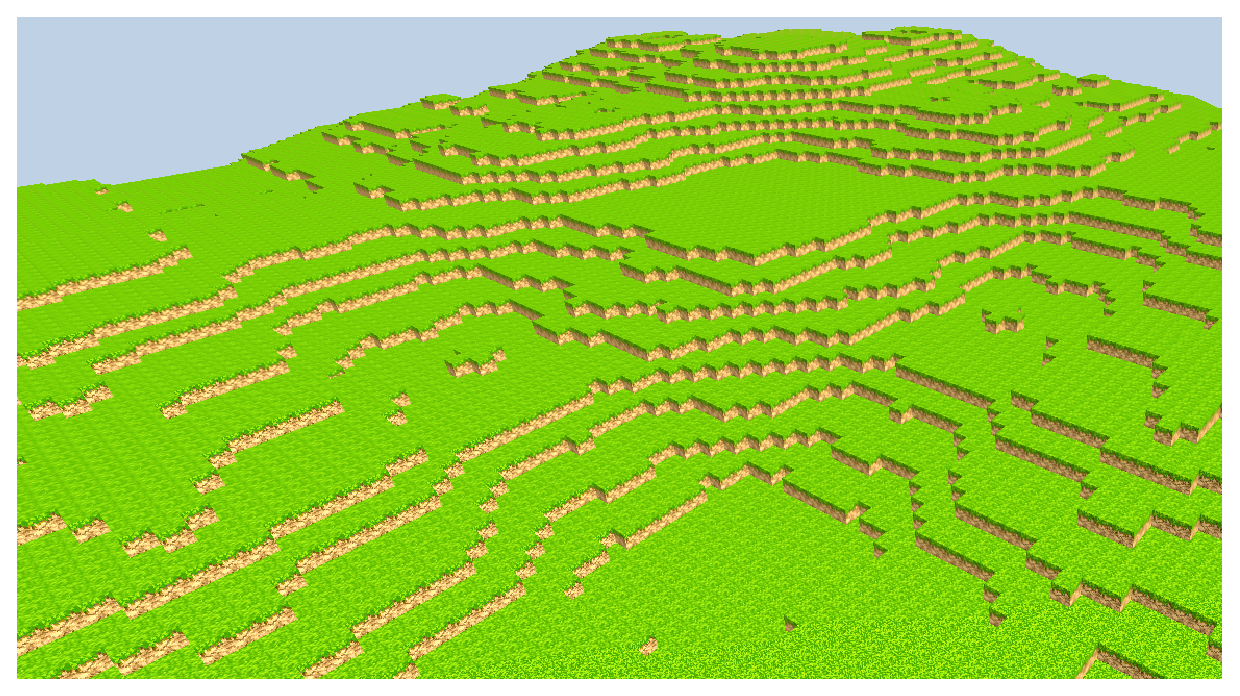
\includegraphics[height=3cm]{images/OurMinecraftWorld.eps}\\
	\textit{Image 9. Ancienne carte.}\\
\end{center}

Cette carte a depuis subi de nombreuses améliorations, tant visuelles que du point de vue de la jouabilité. En effet, lors de la dernière version de ce projet (que nous appellerons V0), nous clôturions le rapport avec une liste d'axes d'améliorations. Nous n'avons eu qu'à piocher dans cette liste au gré des envies afin d'agrémenter le projet de nouveautés, et ainsi lui faire adopter la forme qu'il possède à l'heure actuelle.

\begin{center}
	\null\vspace{0.25cm}
	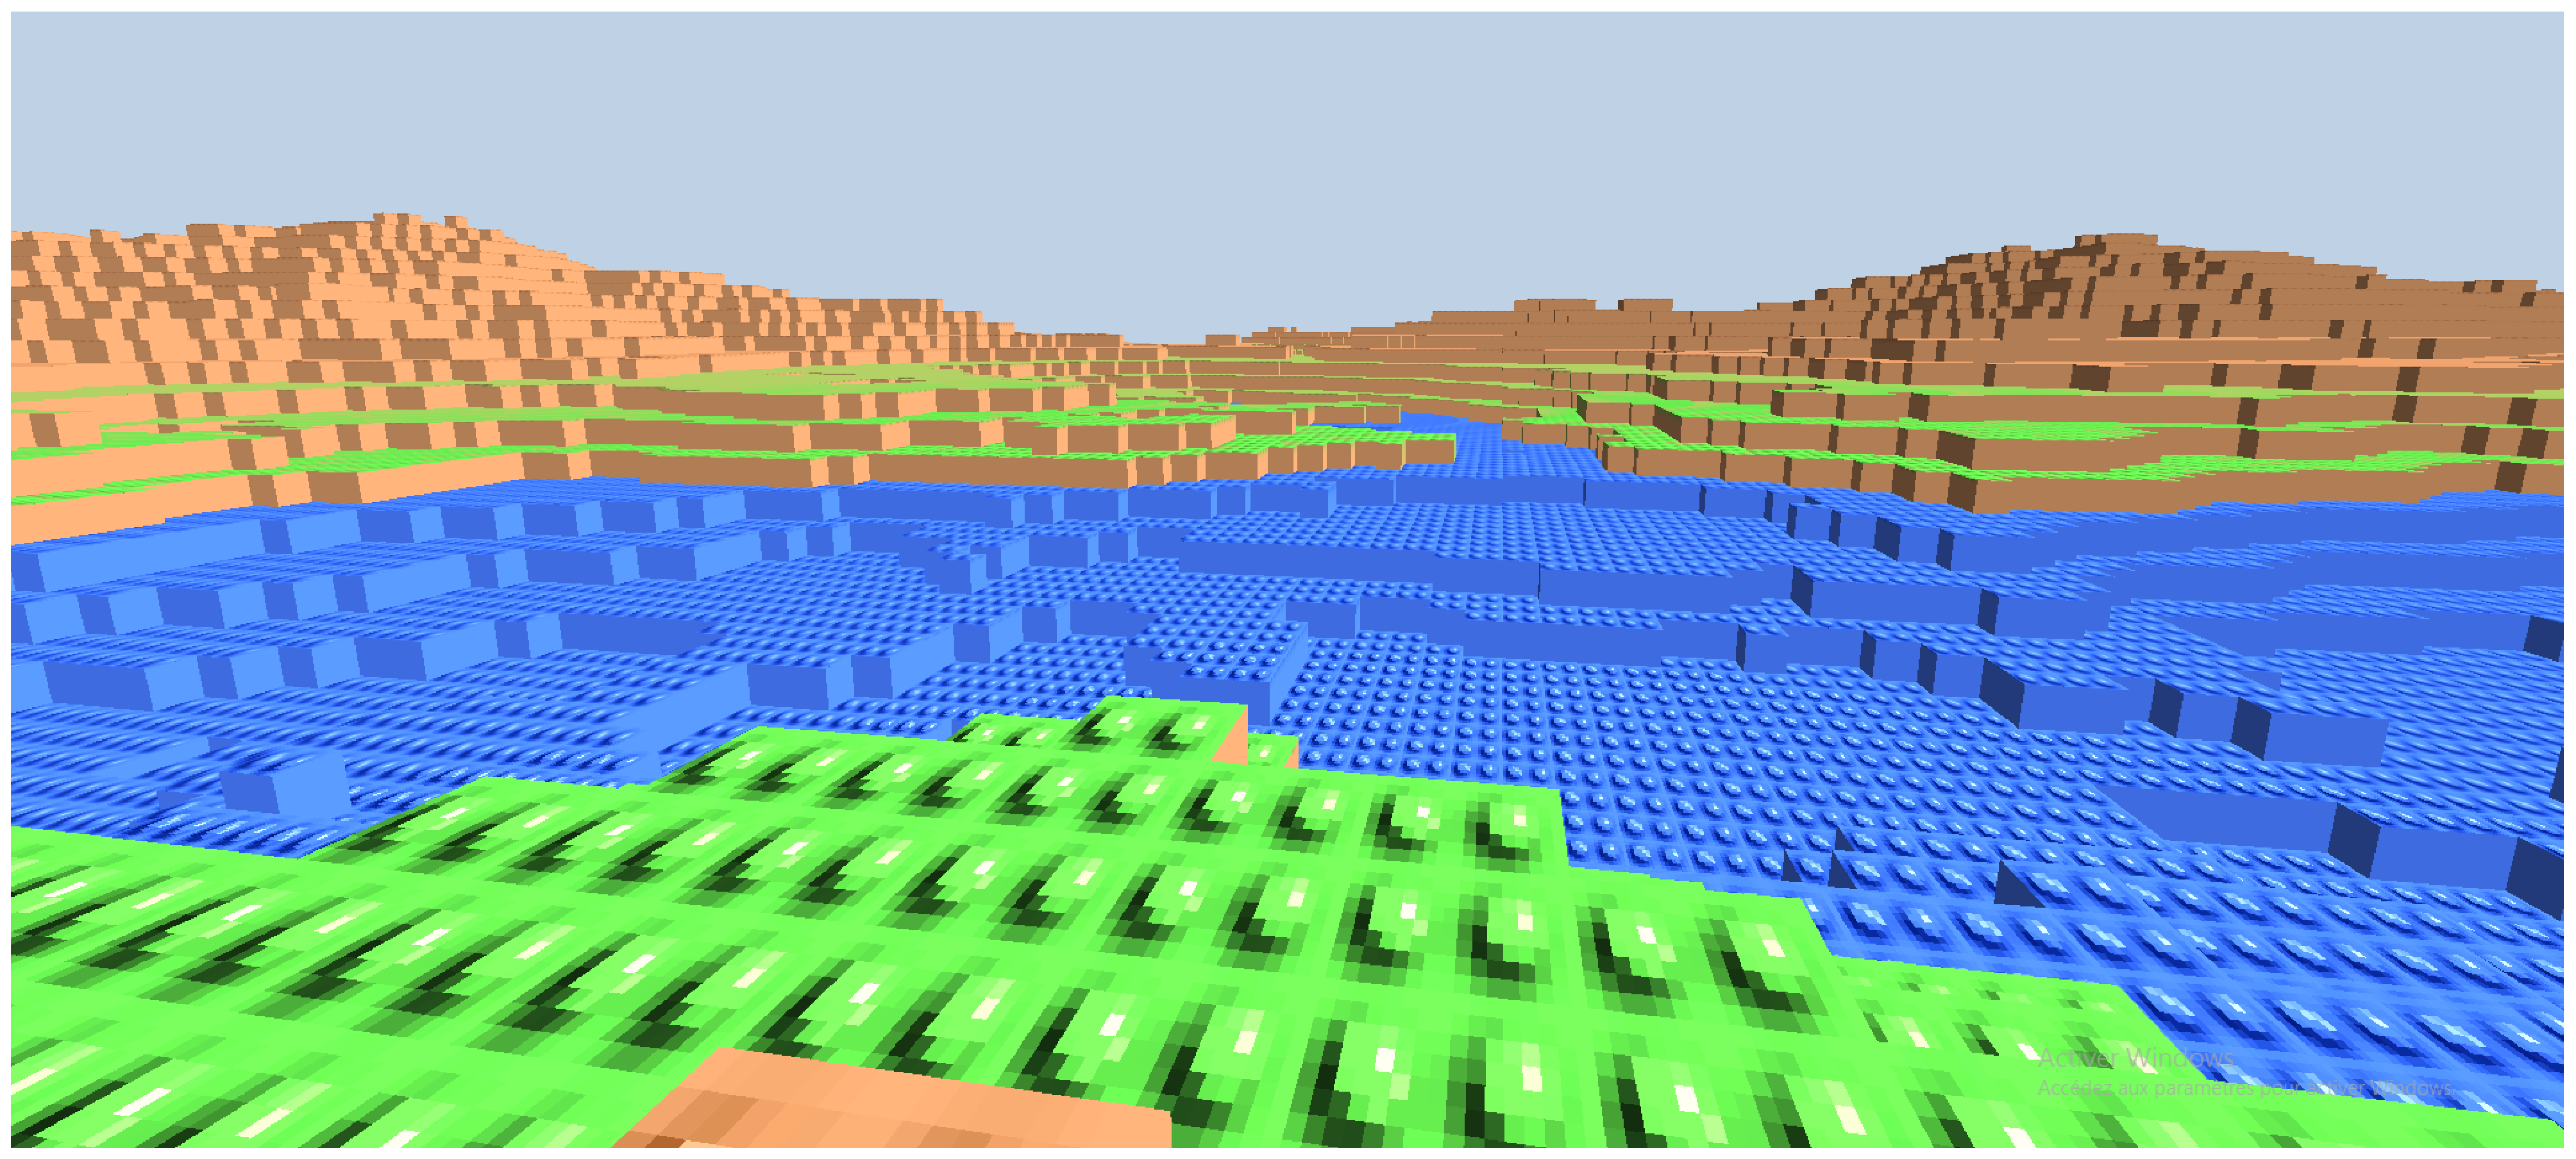
\includegraphics[height=3cm]{images/newworld4.eps}\\
	\textit{Image 10. Nouvelle carte.}\\
\end{center}

Afin d'adopter un rendu visuellement plus proche de ce que nous recherchions, la fabrication de la carte a connu deux ajouts :
\begin{enumerate}
	\item \textbf{Nouvelles textures.}
	\item \textbf{Changement de textures.}
\end{enumerate}

Puisque nous cherchions un rendu visuel proche de Lego et que l'API Three.JS s'inspire de Minecraft, nous avons choisi un pack de textures Minecraft, LegoPack. 
 
\begin{center}
	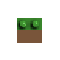
\includegraphics[height=3cm]{images/grass.eps}\\	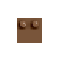
\includegraphics[height=3cm]{images/dirt.eps}\\	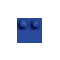
\includegraphics[height=3cm]{images/water.eps}\\
	\textit{Image 11. Aperçu des nouvelles textures.}\\
\end{center}

Ces nouvelles textures remplacent l'ancienne texture unique et uniforme. Puis, afin d'appliquer un peu de variété au relief et d'exploiter au mieux les nouvelles textures, nous avons établi trois niveaux de terrain lors de la génération de la carte par le bruit de Perlin :
\begin{enumerate}
	\item \textbf{La montagne (Hight Layer)}
	\item \textbf{La prairie (Middle Layer)}
	\item \textbf{La mer (Low Layer)}
\end{enumerate}
Le type de terrain varie en fonction de la hauteur de celui-ci. Pour ce faire, lors du calcul initial de la carte, on récupère la hauteur de chaque bloc et on lui applique une texture en fonction de cette valeur.

\begin{center}
	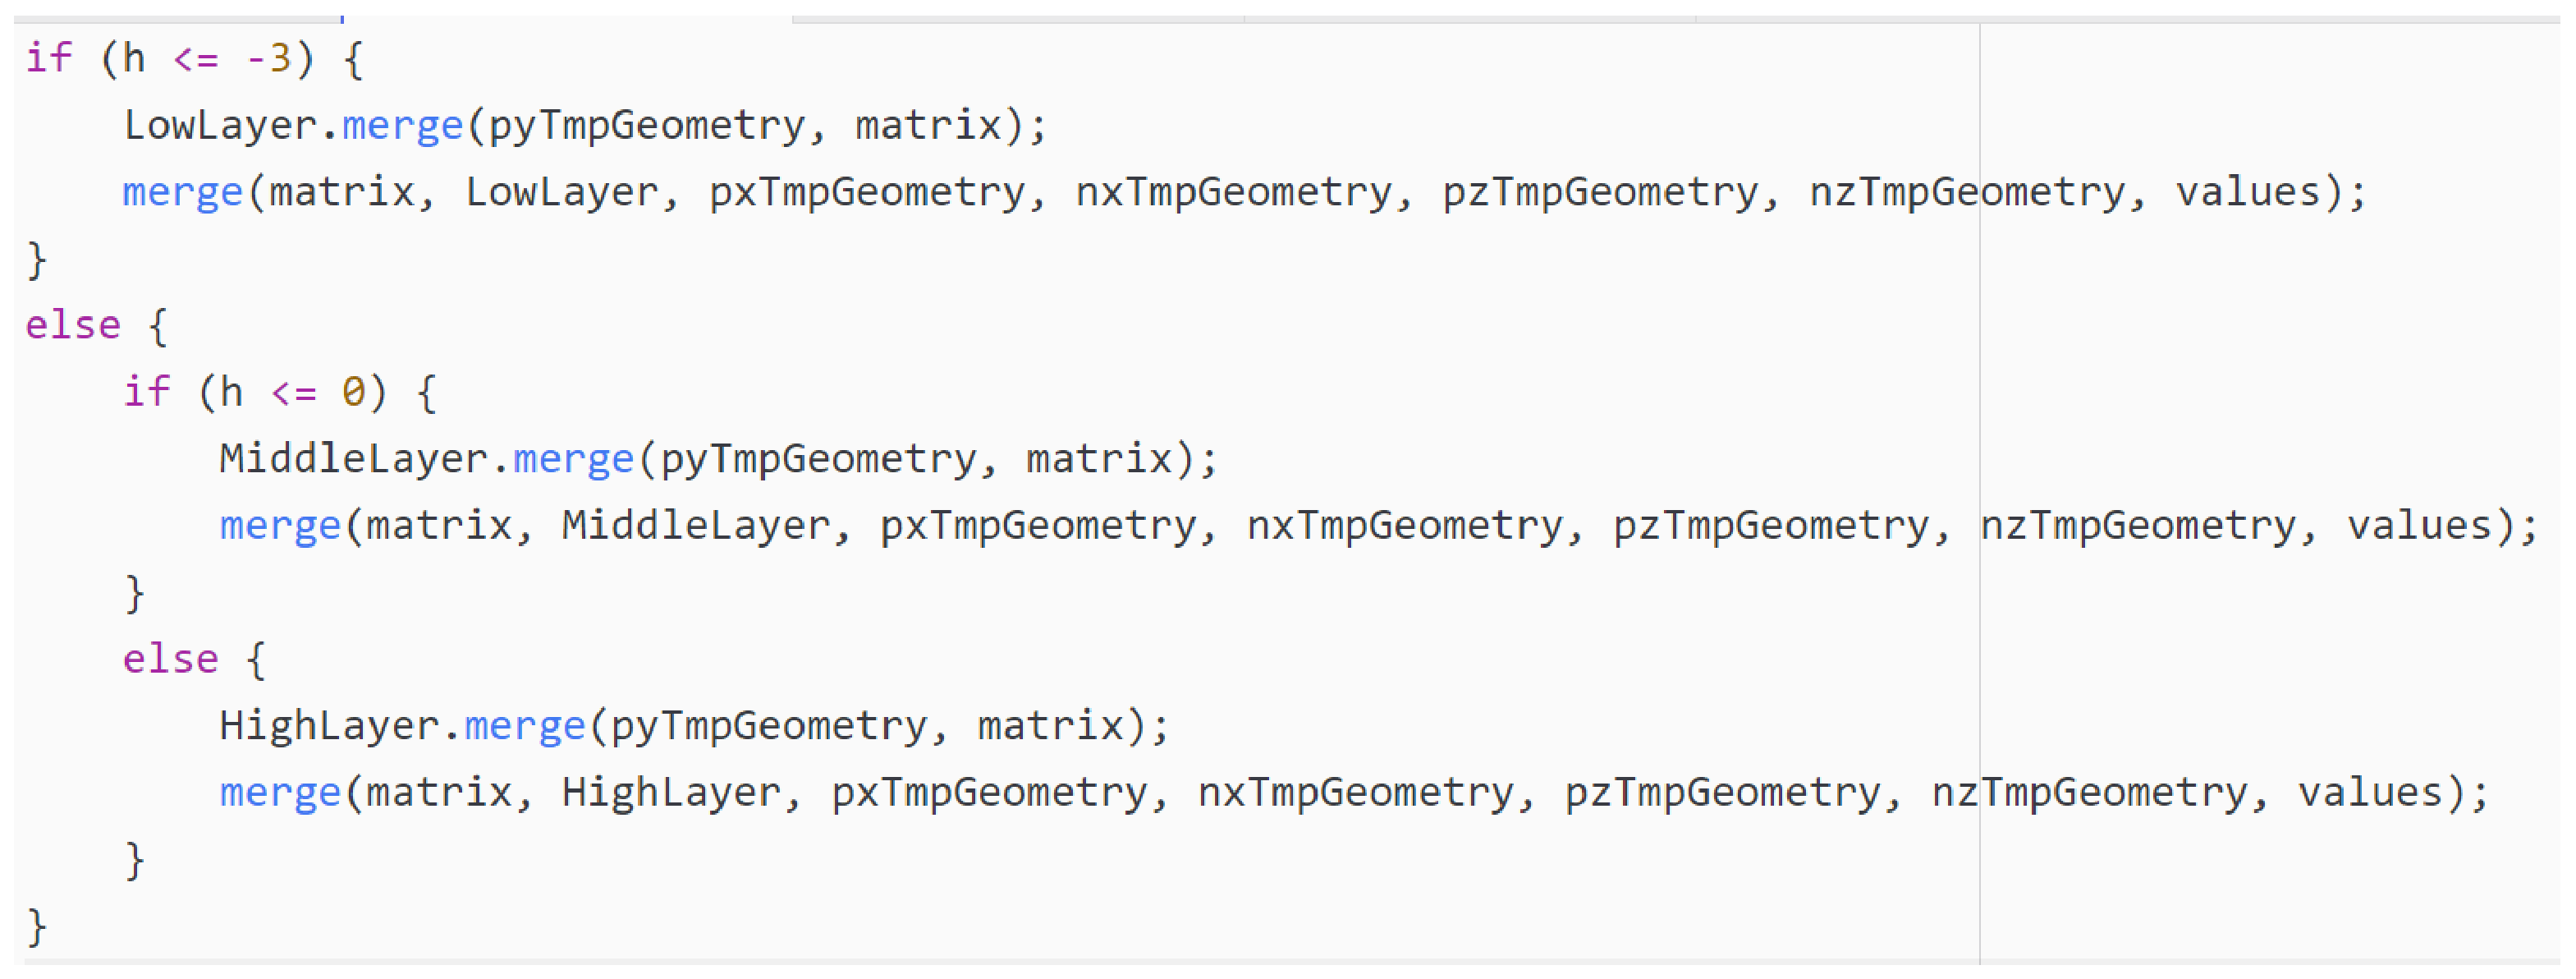
\includegraphics[height=3cm]{images/code_cubes.eps}\\	
	\textit{Extrait de code 1. En fonction de la hauteur du cube, on lui applique une texture différente.}
\end{center}


\section{La physique du terrain}
Par défaut, l'ancienne version de la carte ne possédait pas de physique : la caméra pouvait voler dans toutes les directions et même passer à travers la carte. Désormais, le personnage ne peut se déplacer que sur le sol. 
Désormais, le sol possède une physique et le personnage ne peut pas le traverser. Pour ce faire, il a fallu ajouter un contrôle de la hauteur de la caméra par rapport au cube qu'il est en train de parcourir, et de recalculer sa hauteur en fonction de celle des cubes au sol. 

\begin{center}
	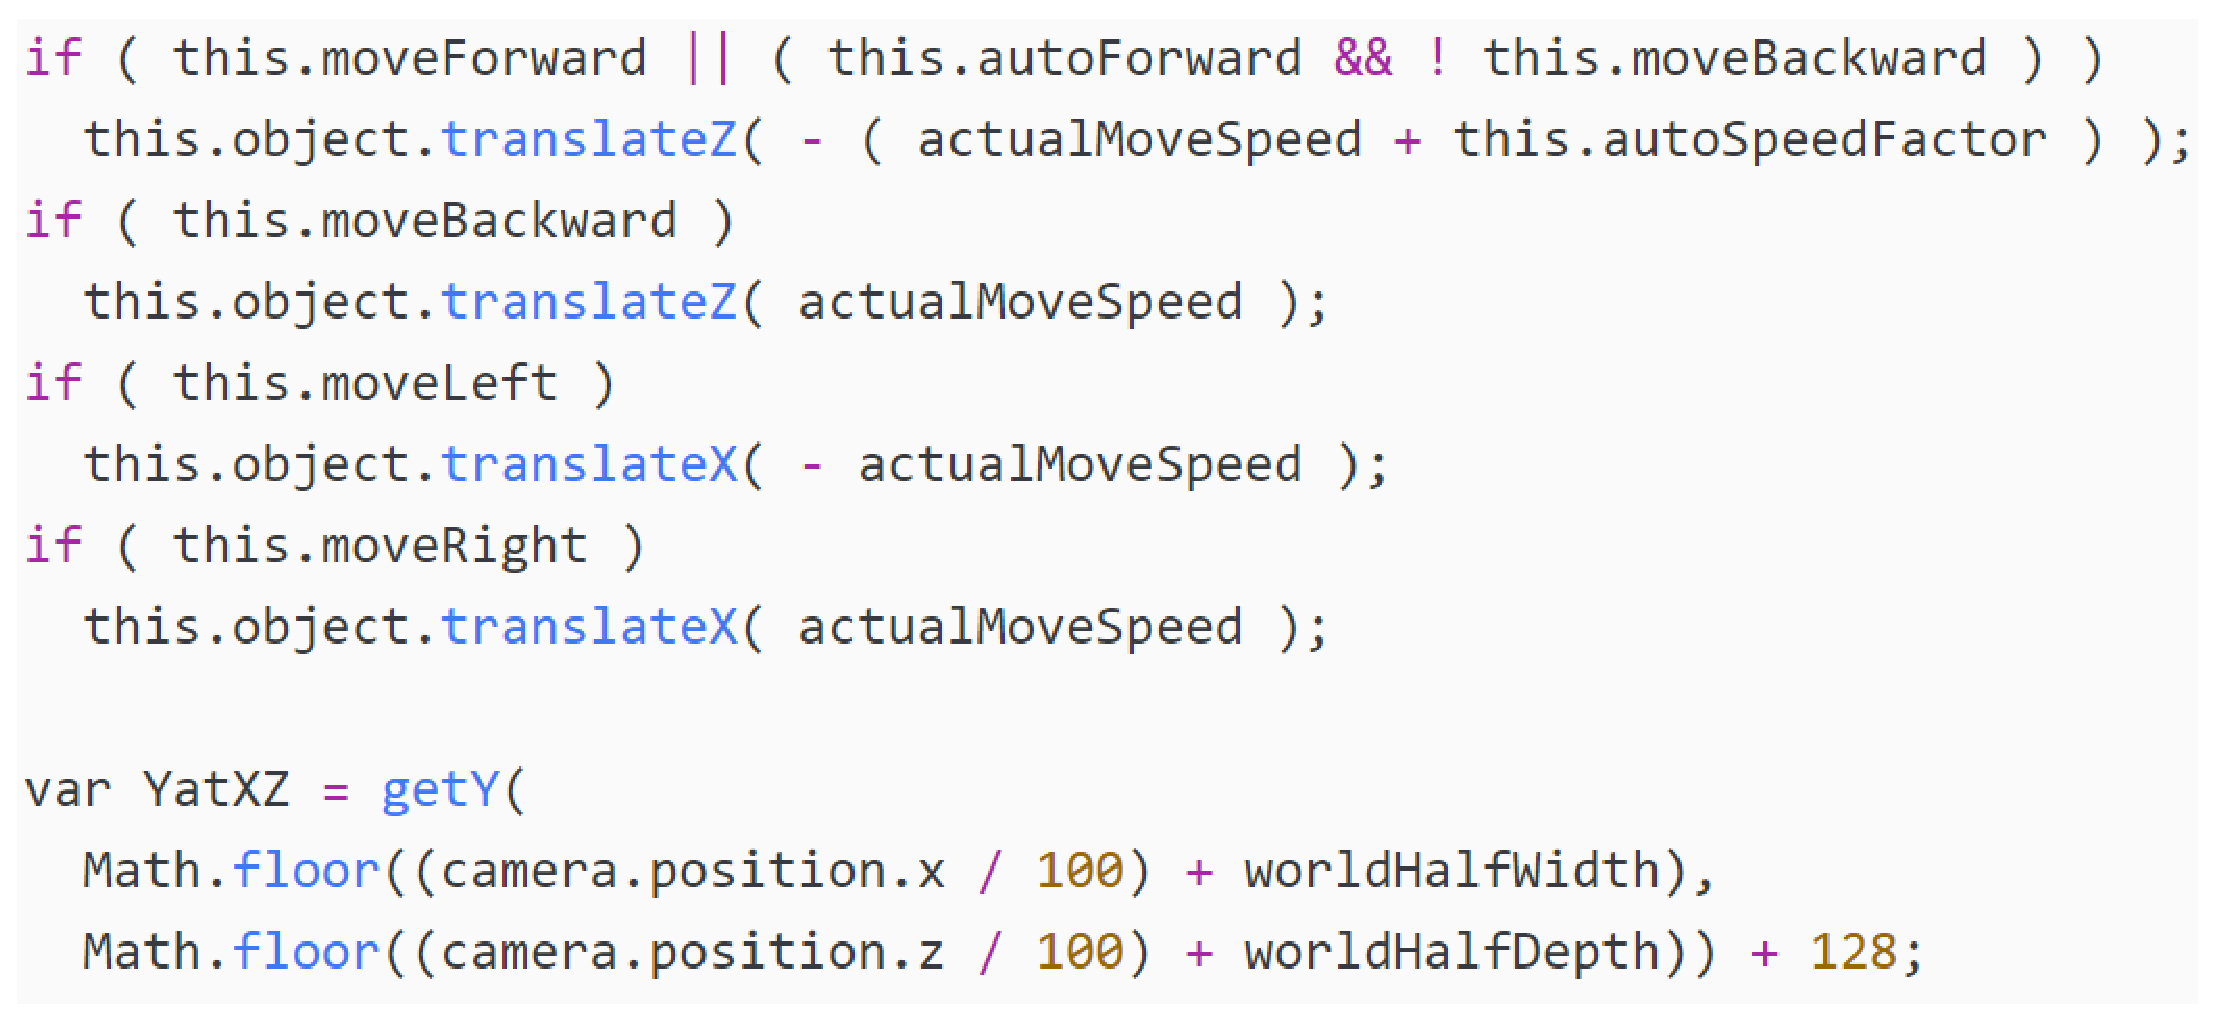
\includegraphics[height=3cm]{images/code_hauteur.eps}\\
	\textit{Extrait de code 2. Gestion de la hauteur du personnage en fonction de sa position à l'intérieur de l'environnement.}
\end{center}


\section{Les contrôles}
L'unde des exigences de la nouvelle version était de refaire les contrôles du jeu. En effet, three.js était par défaut configurée en QWERTY, ce qui rendait les contrôles complexes sur un clavier en AZERTY.
Il faut savoir que dans three.JS, les contrôles sont localisés dans un objet nommé FirstPersonControls. Initialisé pendant la phase de génération du monde, cet objet vérifie les entrées utilisateur et les compare avec une liste d'événements. Les plus importants de ces événements sont onMouseMove (pour calculer la rotation de la caméra), onMouseDown et onMouseUp (quand un clic de la souris est enfoncé puis relâché) et onKeyDown et onKeyUp (même chose pour le clavier.) Lorsque l'un de ces événements survient, le programme récupère le code de la touche enfoncée afin de vérifier si elle correspond à une action.

\begin{center}
	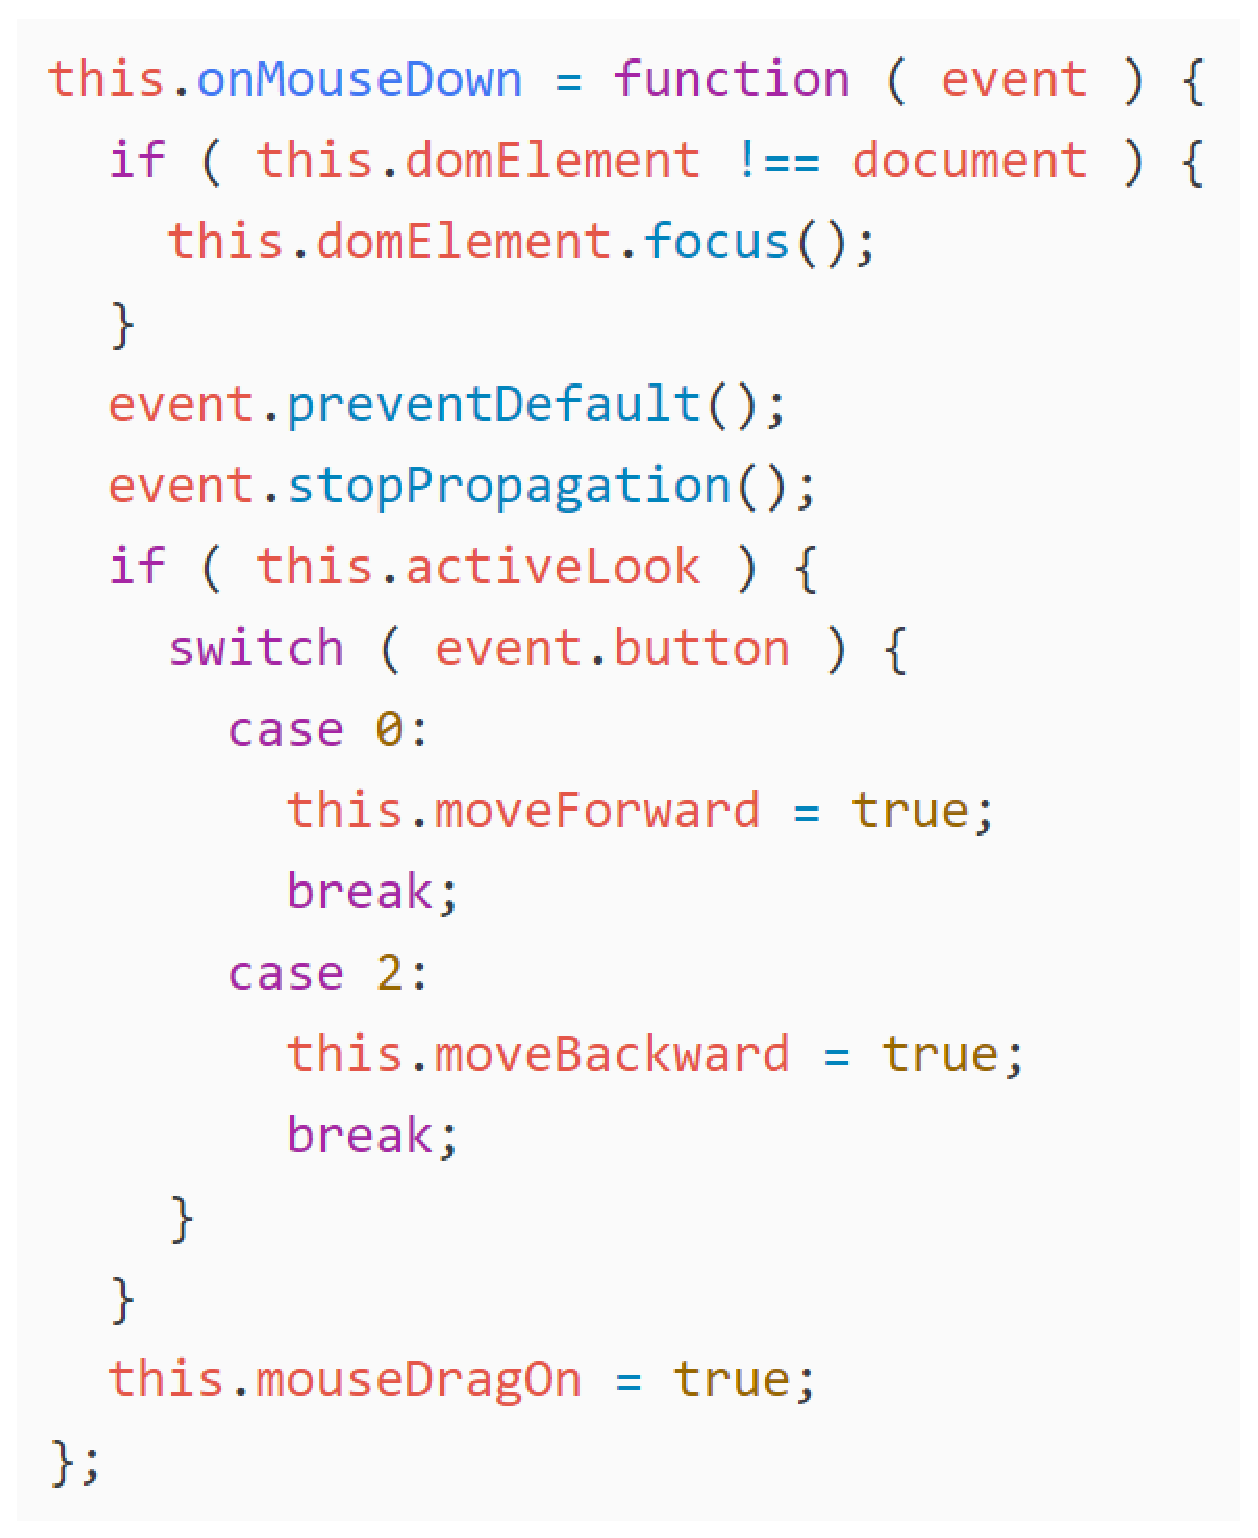
\includegraphics[height=3cm]{images/code_onmousedown.eps}\\
	\textit{Extrait de code 3. Gestion du clic de la souris avec l'événement onMouseDown.}
\end{center}